\documentclass[tikz,border=4pt]{standalone}
\usepackage{amsmath}
\begin{document}
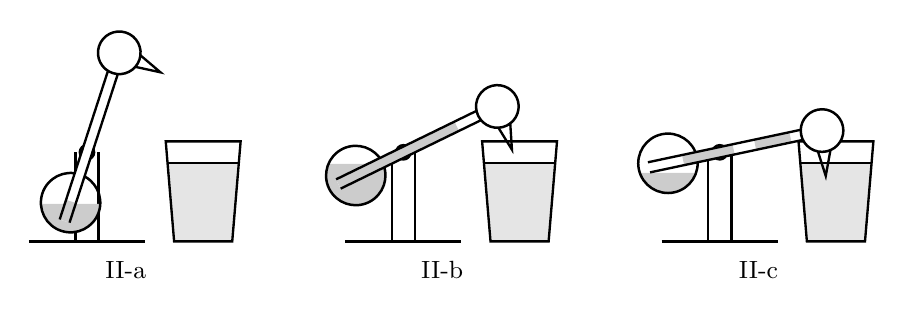
\begin{tikzpicture}[>=stealth, thick, scale=0.82]
  % Panel (a): Initial position (II-a, slight tilt 18 deg)
  \begin{scope}[xshift=-4.6cm]
    % Stand
    \draw[line width=0.85pt] (-0.9, -1.5) -- (0.9, -1.5);
    \draw[line width=0.85pt] (-0.18, -1.5) -- (-0.18, -0.12);
    \draw[line width=0.85pt] (0.18, -1.5) -- (0.18, -0.12);
    \fill[white] (0, -0.12) circle (3.2pt);
    \draw[line width=0.8pt] (0, -0.12) circle (3.2pt);

    % Cup of water on the right
    \fill[gray!20] (1.26, -0.28) -- (1.35, -1.5) -- (2.25, -1.5) -- (2.34, -0.28) -- cycle;
    \draw[line width=0.65pt] (1.26, -0.28) -- (2.34, -0.28);
    \draw[line width=0.85pt] (1.35, -1.5) -- (1.22, 0.05) -- (2.38, 0.05) -- (2.25, -1.5) -- cycle;

    % Bird tilted 18 deg clockwise around pivot (0, -0.12)
    \begin{scope}[shift={(0, -0.12)}, rotate=-18]
      \begin{scope}
        \clip (0, -0.82) circle (0.46);
        \fill[gray!40, rotate=18] (-0.9, -1.4) rectangle (0.4, -0.80);
      \end{scope}
      \draw[line width=0.9pt] (0, -0.82) circle (0.46);
      \fill[white] (-0.08, -1.12) rectangle (0.08, 1.32);
      \fill[gray!40] (-0.08, -1.12) rectangle (0.08, -0.80);
      \draw[line width=0.85pt] (-0.08, -1.12) -- (-0.08, 1.32);
      \draw[line width=0.85pt] (0.08, -1.12) -- (0.08, 1.32);
      \fill[white] (0, 1.62) circle (0.33);
      \draw[line width=0.9pt] (0, 1.62) circle (0.33);
      \draw[line width=0.85pt] (0.31, 1.69) -- (0.70, 1.53) -- (0.30, 1.49);
    \end{scope}
    \node[below, font=\small] at (0.6, -1.65) {$\mathrm{II\text{-}a}$};
  \end{scope}

  % Panel (b): Liquid rises, bird tips forward, beak touches water (II-b, tilt 64 deg)
  \begin{scope}[xshift=0.3cm]
    \draw[line width=0.85pt] (-0.9, -1.5) -- (0.9, -1.5);
    \draw[line width=0.85pt] (-0.18, -1.5) -- (-0.18, -0.12);
    \draw[line width=0.85pt] (0.18, -1.5) -- (0.18, -0.12);
    \fill[white] (0, -0.12) circle (3.2pt);
    \draw[line width=0.8pt] (0, -0.12) circle (3.2pt);

    \fill[gray!20] (1.26, -0.28) -- (1.35, -1.5) -- (2.25, -1.5) -- (2.34, -0.28) -- cycle;
    \draw[line width=0.65pt] (1.26, -0.28) -- (2.34, -0.28);
    \draw[line width=0.85pt] (1.35, -1.5) -- (1.22, 0.05) -- (2.38, 0.05) -- (2.25, -1.5) -- cycle;

    \begin{scope}[shift={(0, -0.12)}, rotate=-64]
      \begin{scope}
        \clip (0, -0.82) circle (0.46);
        \fill[gray!40, rotate=64] (-1.4, -0.85) rectangle (0.2, -0.18);
      \end{scope}
      \draw[line width=0.9pt] (0, -0.82) circle (0.46);
      \fill[white] (-0.08, -1.12) rectangle (0.08, 1.32);
      \fill[gray!40] (-0.08, -1.12) rectangle (0.08, 0.92);
      \draw[line width=0.85pt] (-0.08, -1.12) -- (-0.08, 1.32);
      \draw[line width=0.85pt] (0.08, -1.12) -- (0.08, 1.32);
      \fill[white] (0, 1.62) circle (0.33);
      \draw[line width=0.9pt] (0, 1.62) circle (0.33);
      \draw[line width=0.85pt] (0.31, 1.69) -- (0.70, 1.53) -- (0.30, 1.49);
    \end{scope}
    \node[below, font=\small] at (0.6, -1.65) {$\mathrm{II\text{-}b}$};
  \end{scope}

  % Panel (c): Further tilt (78 deg), tube bottom clears liquid -> vapor bubble enters neck (II-c)
  \begin{scope}[xshift=5.2cm]
    \draw[line width=0.85pt] (-0.9, -1.5) -- (0.9, -1.5);
    \draw[line width=0.85pt] (-0.18, -1.5) -- (-0.18, -0.12);
    \draw[line width=0.85pt] (0.18, -1.5) -- (0.18, -0.12);
    \fill[white] (0, -0.12) circle (3.2pt);
    \draw[line width=0.8pt] (0, -0.12) circle (3.2pt);

    \fill[gray!20] (1.26, -0.28) -- (1.35, -1.5) -- (2.25, -1.5) -- (2.34, -0.28) -- cycle;
    \draw[line width=0.65pt] (1.26, -0.28) -- (2.34, -0.28);
    \draw[line width=0.85pt] (1.35, -1.5) -- (1.22, 0.05) -- (2.38, 0.05) -- (2.25, -1.5) -- cycle;

    \begin{scope}[shift={(0, -0.12)}, rotate=-78]
      \begin{scope}
        \clip (0, -0.82) circle (0.46);
        \fill[gray!40, rotate=78] (-1.5, -0.85) rectangle (0.2, -0.32);
      \end{scope}
      \draw[line width=0.9pt] (0, -0.82) circle (0.46);
      \fill[white] (-0.08, -1.12) rectangle (0.08, 1.32);
      \fill[gray!40] (-0.08, -0.58) rectangle (0.08, 0.22);
      \fill[gray!40] (-0.08, 0.56) rectangle (0.08, 1.12);
      \draw[line width=0.85pt] (-0.08, -1.12) -- (-0.08, 1.32);
      \draw[line width=0.85pt] (0.08, -1.12) -- (0.08, 1.32);
      \fill[white] (0, 1.62) circle (0.33);
      \draw[line width=0.9pt] (0, 1.62) circle (0.33);
      \draw[line width=0.85pt] (0.31, 1.69) -- (0.70, 1.53) -- (0.30, 1.49);
    \end{scope}
    \node[below, font=\small] at (0.6, -1.65) {$\mathrm{II\text{-}c}$};
  \end{scope}
\end{tikzpicture}
\end{document}
